\documentclass[12pt,a4paper,onecolumn,titlepage]{article}

\usepackage[brazil]{babel}
%\usepackage[latin1]{inputenc}
\usepackage[utf8]{inputenc}
\usepackage{graphicx}
\graphicspath{{figuras/}}

\begin{document} %Inicio do documento

\begin{titlepage} %Capa
	
	\vfill
	\begin{center}
	
		{\large \textbf{Faculdade de Ciências e Tecnologia\\Universidade Estadual Paulista\\``Júlio de Mesquita Filho''}} \\[3cm]
		{\large \textbf{Bruno Santos de Lima}}\\
		{\large \textbf{Leandro Ungari Cayres}}\\[4cm]
		{\Large Documento de Requisitos}\\
		{\Large Sistema LearnStation}\\[4cm]

	\hspace{.45\textwidth} %posiciona a minipage
	\begin{minipage}{.5\textwidth}
		\large Disciplina de Engenharia de Software I. Professor Dr. Rogério Eduardo Garcia.\\[0.5cm]
	\end{minipage}

	\vfill
	\vspace{1.5cm}
	
	\large \textbf{Presidente Prudente\\}
	\large \textbf{Abril - 2016}
	
	\end{center}
	
\end{titlepage}
%Fim da capa

%Conteúdo do documento
\section{Introdução}
\label{sect:intro}

\subsection{Propósito do documento de requisitos}

O documento tem como objetivo descrever as perspectivas do produto e suas respectivas funcionalidades, bem como todos os recursos de hardware e software necessários para a elaboração deste, contendo todas as especificações de requisitos necessários. Esta ferramenta não possui um público alvo específico, porém é destinada a aqueles que buscam adquirir e/ou transmitir conhecimento.

\subsection{Escopo do produto}

O sistema busca oferecer um compartilhamento de conhecimento entre pessoas, permitindo a comunicação entre estes através de um mecanismo de conversa, interação entre amigos e participação em cursos tanto como professor ou aluno. Além disso, é possível, sendo professor, disponibilizar o seu próprio curso contendo material textual, questionários e até componentes de mídia.

\subsection{Definições, siglas e abreviaturas}

Segue abaixo, a lista de siglas e abreviaturas utilizadas neste documento:
\begin{itemize}
\item RF: Requisito Funcional
\item RNF: Requisito não Funcional
\end{itemize}

\subsection{Visão geral do documento}

Neste documento serão abordados alguns assuntos como divididos a seguir: na Seção \ref{sect:descricao} é apresentado a descrição geral do produto, assim como suas funcionalidades e respectivas restrições bem como o ambiente de execução. A seguir na Seção \ref{sect:requisitos} é descrito o conjunto de todos os requisitos do sistema e do projeto. %Por fim a Seção \ref{apoio} temos as informações de apoio.

\section{Descrição geral}
\label{sect:descricao}

\subsection{Perspectiva do Produto}

O sistema utiliza uma máquina de servidor que trabalha diretamente com o banco de dados que mantém dados relativos aos usuários, bem como as interações destes realizadas no sistema, com participação em cursos, em ambos papéis e suas interações com outros usuários.

\subsection{Funções do Produto}


O sistema permite que os usuários realizem inscrição em um ou mais cursos de diversas temáticas, sendo que estes cursos foram elaborados por outros usuários, que desta forma atuam no papel de professor. Os cursos são compostos por aulas, cujo conteúdo destas abrange tanto materiais textuais quando recursos de multimídia. Os usuários podem relacionar-se enviando solicitações de amizade, em que a partir do momento em que ambos são amigos eles também podem comunicar-se através de conversas.


\begin{figure}[!htb]
  \centering
  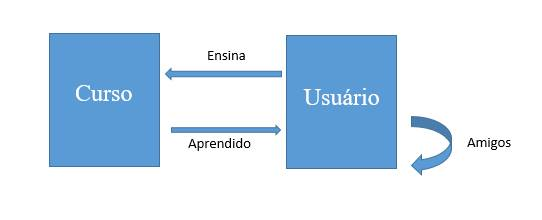
\includegraphics[scale=0.7]{figura1.png}
  \caption{Funcionamento da rede social de cursos}
  \label{figRotulo}
\end{figure}


\subsection{Caracteristicas do Usuário}

O usuários do sistema tem como características o interesse em transmitir ou adquirir conhecimentos sobre uma temática especifica, podendo também interagir com os demais usuários afim de potencializar o conhecimento adquirido.

\subsection{Restrições}

O sistema será desenvolvido para plataforma web, desta forma sendo acessível tanto por desktop ou por dispositivos móveis, sendo que este último tem maiores restrições de hardware e determinados conteúdos relacionados aos cursos, especificamente conteúdos de multimídia, podem ter sua execução impedida ou desempenho reduzido devido a essas limitações.

Em relação ao restante do projeto, este se utiliza das recentes tecnologias de desenvolvimento web, logo usuários que possuirem navegadores desatualizados poderão enfrentar algumas dificuldades.

\subsection{Suposições e Dependências}

Este software não possui nenhuma limitação quanto ao sistema operativo ou hardware.

\section{Requisitos Específicos}
\label{sect:requisitos}

%\subsection{Interfaces Externas} Poderia usar um sistema externo para criptografar contas de usuarios ou o facebook para criar contas de usuários.

\subsection{Requisitos Funcionais}

\begin{description}

%RF. 1: Usuário.

\item RF. 1.1: Registrar a inscrição do usuário. (E)
\item \qquad Informações do usuário: Nome completo, data de nascimento, e-mail, senha, país onde reside, gênero.

\item RF. 1.2: Busca e listagem de usuários. (E)
\item \qquad A busca será realizada por nome de usuário.

\item RF. 1.3: Exibir perfil de usuário que foi buscado. (E)
\item \qquad Serão exibidas informações de identificação e contato do usuário.

\item RF. 1.4: Enviar e responder solicitação de amizade. (E)
\item \qquad Para o envio será especificado o usuário tais como o dia e a hora em que foram solicitados, e para a resposta a confirmação ou não além do horário da operação.

\item RF. 1.5: Cancelamento de amizade.(E)
\item \qquad Neste quesito o cancelamento de amizade ocorre de forma mútua.

\item RF. 1.6: Busca e listagem de cursos. (E)
\item \qquad Os cursos são buscados por nome e área de conhecimento.
 
\item RF. 1.7: Inscrição em Curso. (E)
\item \qquad O usuário efetua a inscrição no curso e passa a ter acesso ao conteúdo do curso por completo.

\item RF. 1.8: Cancelamento de Inscrição em Curso. (E)
\item \qquad O usuário efetua o cancelamento passando a não ter mais acesso ao conteúdo das aulas e perde seu progresso no mesmo.

\item RF. 1.9: Criar Curso. (E)
\item \qquad O usuário pode criar um curso, passando a ser professor deste, fornecendo as seguintes informações: nome do curso, área de conhecimento, nível de complexidade (básico, intermediário e avançado).

\item RF. 1.10: Avaliar qualidade de cursos. (E)
\item \qquad O usuário pode avaliar a qualidade do curso em que está inscrito, sendo esta qualidade classificada por no maxímo 5 estrelas.

%Não é viagem, não este mecanismo não será externo mas sim interno, pesquisar por md5 php
\item RF. 1.11: Prover maior segurança das informações dos usuários. (O)
\item \qquad Será realiza a criptografia da senha dos usuários.

\item RF. 1.12: Enviar e receber mensagens para um amigo. (E)
\item \qquad As mensagens podem ser trocadas entre dois usuários sempre na forma de textos.

%\item RF. 1.13: Notificação de recebimento de uma mensagem de um amigo. (E)
%\item \qquad O usuário é notificado que recebeu uma mensegem de um determinado amigo.

%\item RF. 1.14: Notificações de informação, na forma de aviso de aulas novas inseridas no curso em que está %inscrito ou de solicitação de amizade. (E)

\item RF. 1.13: Notificações recebidas. (E) 
\item \qquad O usuário será notificado nas seguintes condições:
\item \qquad O usuário é notificado que recebeu uma mensegem de um determinado amigo.
\item \qquad Atualização de conteúdo dos cursos.
\item \qquad Novas solicitações de amizades.

\item RF. 1.14: Encerramento de conta de usuário. (E)
\item \qquad O usuário pode encerrar sua conta na rede social.

\item RF. 1.15: Remover informações relacionados ao usuário excluído. (O)
\item \qquad Após a exclusão de uma conta de usuário, serão também removidas todas as relações de amizade, cursos criados por este, consequentemente as inscrições de outros usuários nesses cursos; as inscrições em cursos realizadas pelo usuário removido e todas as conversas desse usuário.

\item RF. 1.16: Denunciar possível conteúdo inadequado. (E)
\item \qquad O usuário ao identificar algum tipo de conteúdo inadequado, ou seja, um conteúdo que possua linguagem inadequada, infrinjam leis locais, promovam preconceitos e/ou induzam a violência, poderá realizar uma denúncia ao administrador.

%RF. 2: Curso.
\item RF. 2.1: Adicionar uma aula a um determinado curso. (E)
\item \qquad As aulas podem ser adicionadas ao curso na forma de documentos textuais e/ou conteúdo de mídia, além de exercícios na forma de formularios.

\item RF. 2.2: Exibir descrição do curso. (E)
\item \qquad Seram exibidas informações referentes ao curso, tais como: nome do curso, área de conhecimento, professor do curso, nota de avaliação do curso, lista de aulas.

\item RF. 3.1: Acesso a listagem de todos os conteúdos. (E)
\item \qquad O usuário com permissão de administrador terá acesso a listagem de todos os usuários, cursos criados e aulas incluidas além de seus respectivos conteúdos.

\item RF. 3.2: Remoção de conteúdos classificados inadequados. (E)
\item \qquad O usuário com permissão de administrador poderá excluir definitivamente conteúdos presentes em conversas, cursos, contas de usuários ou informações pessoais em perfis que possuam linguagem inadequada, infrinjam leis locais, promovam preconceitos e/ou induzam a violência de forma que este julgar pertinente.

\item RF. 3.3: Envio de notificação de advertência ao usuário.(E)
\item \qquad O usuário com permissão de administrador poderá enviar advertências, caso julgue pertinente perante o uso inadequado do sistema, sendo possivel o banimento deste, caso justificado.


\end{description}

\subsection{Requisitos Não Funcionais}

\qquad RNF. 1: O sistema será desenvolvido para a plataforma web utilizando como linguagem de programação o PHP, além de linguagem de marcação HTML, CSS, assim como utilizando JavaScript.\\

RNF. 2: Para utilizar o sistema basta utilizar um software para navegação na internet e utilizar um endereço para comunicação com o servidor em que o sistema está rodando e assim começar a utilizar a rede social LearnStation.\\

RNF. 3: Para o armazenamento dos dados será utilizado o Sistema de Gerenciamento de Banco de Dados MySQL.\\

%Possivel ideia de uma interface externa
%RNF: 4: A rede social vai utilizar um sistema externo de criptografia para realização de login e logout por parte dos usuarios %afim de prover uma maior segurança.\\

%\subsection{Requisitos Desempenho}
%\subsection{Requisitos Lógicos de Banco de Dados}
%\subsection{Restrições de Projeto}
%\subsection{Atributo do Sistema de Software}



%\subsection{Organização}
%\section{Informações de Apoio}
%\label{apoio}
  
  
%\subsection{Índice}
%\label{indice}

\renewcommand{\contentsname}{Índice}
\tableofcontents

%\section{Apêndices}
%\label{sect:apendices}

%Fim do conteúdo do documento
%referencias - estilos: http://www.cs.stir.ac.uk/~kjt/software/latex/showbst.html
%\bibliographystyle{acm}
%\bibliography{referencias}

\end{document} %Fim do documento
